% Active cells of the 3 x 3 array at each step. PE(i,j) is active for
% i+j <= t <= i+j+2. The same pattern is checked against the RTL after
% every clock edge by tb_systolic_array.v.
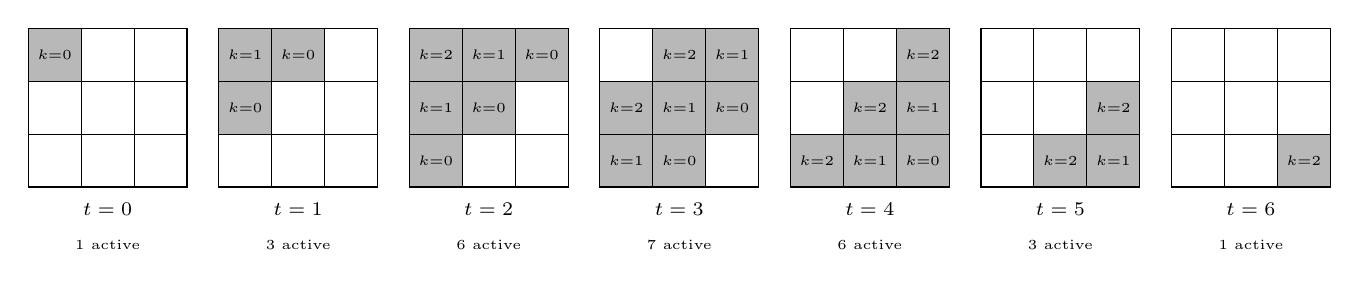
\begin{tikzpicture}[font=\scriptsize, x=0.42cm, y=0.42cm]
  \foreach \t in {0,...,6} {
    \begin{scope}[xshift=\t*2.42cm]
      \foreach \i in {0,1,2} {
        \foreach \j in {0,1,2} {
          \pgfmathtruncatemacro{\lo}{\i+\j}
          \pgfmathtruncatemacro{\hi}{\i+\j+2}
          \pgfmathtruncatemacro{\k}{\t-\i-\j}
          \ifnum\t<\lo
            \draw[line width=0.4pt] (\j*1.6,-\i*1.6) rectangle ++(1.6,-1.6);
          \else\ifnum\t>\hi
            \draw[line width=0.4pt] (\j*1.6,-\i*1.6) rectangle ++(1.6,-1.6);
          \else
            \draw[line width=0.4pt, fill=black!28] (\j*1.6,-\i*1.6) rectangle ++(1.6,-1.6);
            \node[font=\tiny] at (\j*1.6+0.8,-\i*1.6-0.8) {$k{=}\k$};
          \fi\fi
        }
      }
      \pgfmathtruncatemacro{\busy}{(\t<3) ? (\t+1)*(\t+2)/2 : ((\t==3) ? 7 : (7-\t)*(8-\t)/2)}
      \node[anchor=north] at (2.4,-5.0) {$t=\t$};
      \node[anchor=north, font=\tiny] at (2.4,-6.1) {\busy\ active};
    \end{scope}
  }
\end{tikzpicture}
